\subsection{Guadagno Open Loop}

In questa ultima parte dell'esperienza abbiamo cercato di misurare il guadagno $A_{ol}$ del nostro amplificatore reale. Come sappiamo, tale guadagno è una funzione della frequenza. Dobbiamo dunque trovare un modo per misurarlo.

\subsubsection{Misura per basse frequenze}

\begin{wrapfigure}[17]{r}{0.55\textwidth}
  \begin{center}
    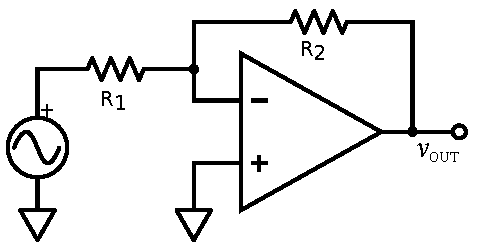
\includegraphics[width=0.280\textwidth]{../E03/latex/HF_ol.pdf}
  \end{center}
  \caption{...}
  \label{cir3:low_frequency}
\end{wrapfigure}


Fino alla frequenza di circa \SI{8}{\hertz} il guadagno di un op-amp $\mu$A741 è di circa $3\times 10^5$. Oltre tale frequenza abbiamo una caduta di circa 20dB/decade. Non risulta dunque possibile effettuare misure a loop aperto in quanto piccolissime variazioni di tensione ai due ingressi causerebbero grandi effetti in uscita. Abbiamo dunque progettato un circuito per ridurre il guadagno in uscita così da non mandare in saturazione il nostro op-amp. In figura (\ref{cir3:low_frequency}) è riportato lo schema circuitale.  

Utilizzando l'oscilloscopio abbiamo misurato i valori di tensione $V_A$ e $V_{out}$. Cerchiamo dunque di legare il guadagno a tali quantità.



